\documentclass[14pt, twoside]{report}

\usepackage[margin=1in]{geometry}
\usepackage{graphicx}
\usepackage{svg}
\usepackage[font={small, it}]{caption}
\usepackage{subcaption}
\usepackage[bookmarks]{hyperref}
\usepackage{minted}
\usepackage[inline]{enumitem}

\svgpath{images/}

\title{\large Something something something \\ Institue Name}
\author{Tejas Sanap}

\begin{document}

\maketitle
\tableofcontents
\listoffigures

\chapter{Chapter of the unknown}

\section{Section of the Unseen}

The Big Bang theory is a cosmological model for the observable universe from the earliest known periods through its subsequent large-scale evolution. The model describes how the universe expanded from a very high-density and high-temperature state, and offers a comprehensive explanation for a broad range of phenomena, including the abundance of light elements, the cosmic microwave background (CMB), large-scale structure and Hubble's law (the farther away galaxies are, the faster they are moving away from Earth). If the observed conditions are extrapolated backwards in time using the known laws of physics, the prediction is that just before a period of very high density there was a singularity which is typically associated with the Big Bang. Current knowledge is insufficient to determine if the singularity was primordial.

Georges Lemaître first noted in 1927 that an expanding universe could be traced back in time to an originating single point, calling his theory that of the "primeval atom". The scientific community was once divided between supporters of two different theories, the Big Bang and the steady state theory, but a wide range of empirical evidence has strongly favored the Big Bang which is now universally accepted. In 1929, from analysis of galactic redshifts, Edwin Hubble concluded that galaxies are drifting apart; this is important observational evidence for an expanding universe. In 1964, the cosmic microwave background radiation was discovered, which was crucial evidence in favor of the hot Big Bang model, since that theory predicted the existence of background radiation throughout the universe before it was discovered.

The known physical laws of nature can be used to calculate the characteristics of the universe in detail back in time to an initial state of extreme density and temperature. Detailed measurements of the expansion rate of the universe place the Big Bang at around 13.8 billion years ago, which is thus considered the age of the universe. After its initial expansion, the universe cooled sufficiently to allow the formation of subatomic particles, and later atoms. Giant clouds of these primordial elements (mostly hydrogen, with some helium and lithium) later coalesced through gravity, eventually forming early stars and galaxies, the descendants of which are visible today. Astronomers also observe the gravitational effects of dark matter surrounding galaxies. Most of the matter in the universe seems to be in the form of dark matter, and the Big Bang theory and various observations indicate that it is not conventional baryonic matter (atoms). It is still not known exactly what dark matter is. More recently, measurements of the redshifts of supernovae indicate that the expansion of the universe is accelerating, an observation attributed to dark energy's existence.

\begin{figure}[h]
	\centering
	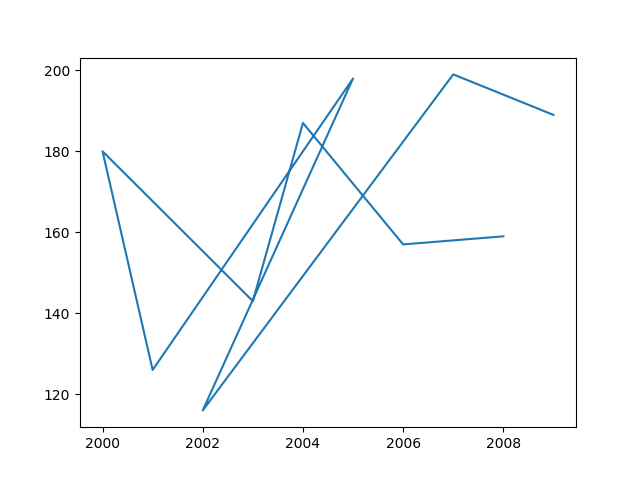
\includegraphics[height=0.3\textheight, keepaspectratio]{images/plot1.png}
	\caption{some random plot}
	\label{fig1}
\end{figure}

\begin{figure}[h]
	\centering
	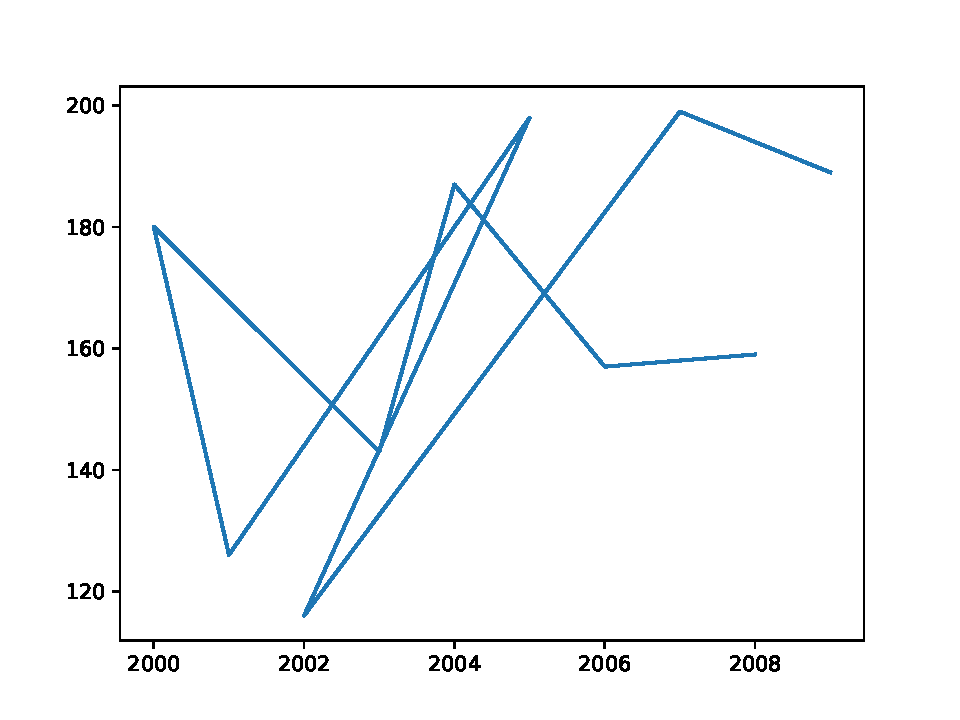
\includegraphics[height=0.3\textheight, keepaspectratio]{images/plot1.pdf}
	\caption{some random plot 2}
	\label{fig2}
\end{figure}

\begin{figure}[h]
	\begin{subfigure}{0.5\textwidth}
		\includesvg[width=\textwidth]{cmbr.svg}
		\caption{Figure 1}
	\end{subfigure}
	\begin{subfigure}{0.4\textwidth}
		\includesvg[width=\textwidth]{PowerSpectrumExt.svg}
		\caption{Figure 3}
	\end{subfigure}
	\caption{Main Figure}
\end{figure}
	
\end{document}
